\documentclass[portrait,final]{baposter}
%\documentclass[a4shrink,portrait,final]{baposter}
% Usa a4shrink for an a4 sized paper.

\tracingstats=2

%% Language and babel
\usepackage[utf8]{inputenc}
\usepackage[T1]{fontenc}
\usepackage[english,french,italian]{babel}

\usepackage{mdwlist}
\usepackage{times}
\usepackage{calc}
\usepackage{relsize}
\usepackage{multirow}
\usepackage{bm}

%% Images
\usepackage{float}
\usepackage{graphicx}
\usepackage{wrapfig}
\usepackage{cclicenses}

%% Layout
\usepackage{multicol}
\usepackage{pgfbaselayers}
\pgfdeclarelayer{background}
\pgfdeclarelayer{foreground}
\pgfsetlayers{background,main,foreground}

\usepackage{helvet}
\usepackage{palatino}

\newcommand{\captionfont}{\footnotesize}

\selectcolormodel{cmyk}

\graphicspath{{images/}}

%%%%%%%%%%%%%%%%%%%%%%%%%%%%%%%%%%%%%%%%%%%%%%%%%%%%%%%%%%%%%%%%%%%%%%%%%%%%%%%%
% Multicol Settings
%%%%%%%%%%%%%%%%%%%%%%%%%%%%%%%%%%%%%%%%%%%%%%%%%%%%%%%%%%%%%%%%%%%%%%%%%%%%%%%%
\setlength{\columnsep}{0.8em}
\setlength{\columnseprule}{0mm}


%%%%%%%%%%%%%%%%%%%%%%%%%%%%%%%%%%%%%%%%%%%%%%%%%%%%%%%%%%%%%%%%%%%%%%%%%%%%%%%%%
%% Save space in lists. Use this after the opening of the list
%%%%%%%%%%%%%%%%%%%%%%%%%%%%%%%%%%%%%%%%%%%%%%%%%%%%%%%%%%%%%%%%%%%%%%%%%%%%%%%%%
%\newcommand{\compresslist}{%
%\setlength{\itemsep}{1pt}%
%\setlength{\parskip}{0pt}%
%\setlength{\parsep}{0pt}%
%}


%%%%%%%%%%%%%%%%%%%%%%%%%%%%%%%%%%%%%%%%%%%%%%%%%%%%%%%%%%%%%%%%%%%%%%%%%%%%%%
%%% Begin of Document
%%%%%%%%%%%%%%%%%%%%%%%%%%%%%%%%%%%%%%%%%%%%%%%%%%%%%%%%%%%%%%%%%%%%%%%%%%%%%%

\begin{document}

%%%%%%%%%%%%%%%%%%%%%%%%%%%%%%%%%%%%%%%%%%%%%%%%%%%%%%%%%%%%%%%%%%%%%%%%%%%%%%
%%% Here starts the poster
%%%---------------------------------------------------------------------------
%%% Format it to your taste with the options
%%%%%%%%%%%%%%%%%%%%%%%%%%%%%%%%%%%%%%%%%%%%%%%%%%%%%%%%%%%%%%%%%%%%%%%%%%%%%%
% Define some colors
\definecolor{silver}{cmyk}{0,0,0,0.3}
\definecolor{yellow}{cmyk}{0,0,0.9,0.0}
\definecolor{reddishyellow}{cmyk}{0,0.22,1.0,0.0}
\definecolor{black}{cmyk}{0,0,0.0,1.0}
\definecolor{darkYellow}{cmyk}{0,0,1.0,0.5}
\definecolor{darkSilver}{cmyk}{0,0,0,0.1}

\definecolor{lightyellow}{cmyk}{0,0,0.3,0.0}
\definecolor{lighteryellow}{cmyk}{0,0,0.1,0.0}
\definecolor{lighteryellow}{cmyk}{0,0,0.1,0.0}
\definecolor{lightestyellow}{cmyk}{0,0,0.05,0.0}

%%
\typeout{Poster Starts}
\background{
  \begin{tikzpicture}[remember picture,overlay]%
    \draw (current page.north west)+(-2em,2em) node[anchor=north west] {
\includegraphics[height=1.1\textheight]{silhouettes_background}};
  \end{tikzpicture}%
}

\newlength{\leftimgwidth}
\begin{poster}%
  % Poster Options
  {
  % Show grid to help with alignment
  grid=no,
  % Column spacing
  colspacing=1em,
  % Color style
  bgColorOne=lighteryellow,
  bgColorTwo=lightestyellow,
  borderColor=reddishyellow,
  headerColorOne=yellow,
  headerColorTwo=reddishyellow,
  headerFontColor=black,
  boxColorOne=lightyellow,
  boxColorTwo=lighteryellow,
  % Format of textbox
  textborder=roundedleft,
  % Format of text header
  eyecatcher=no,
  headerborder=open,
  headerheight=0.08\textheight,
  headershape=roundedright,
  headershade=plain,
  headerfont=\Large\textsf, %Sans Serif
  boxshade=plain,
%  background=shade-tb,
  background=plain,
  linewidth=2pt
  }
  % Eye Catcher
  {\includegraphics[width=10em]{D1077}} % No eye catcher for this poster. (eyecatcher=no above). If an eye catcher is present, the title is centered between eye-catcher and logo.
  % Title
  {\sf %Sans Serif
  %\bf% Serif
  L'impiego di \emph{mobile GIS} open source in Archeologia}
  % Authors
  {\sf %Sans Serif
  % Serif
  \vspace{1em}Francesco de Virgilio \\ \small{Università degli Studi di Bari - Dipartimento Geomineralogico \{fradeve11@gmail.com\}}
  }
  % University logo
  {% The makebox allows the title to flow into the logo, this is a hack because of the L shaped logo.
    \makebox[10em][r]{%
      \begin{minipage}{19em}
        \hfill
        
\includegraphics[height=7.0em]{logo}\hspace{0.3em}
        
\includegraphics[height=7.0em]{logogenerale}
      \end{minipage}
    }
  }

  \tikzstyle{light shaded}=[top color=baposterBGtwo!30!white,bottom color=baposterBGone!30!white,shading=axis,shading angle=30]

  % Width of left inset image
     \setlength{\leftimgwidth}{0.78em+8.0em}

%%%%%%%%%%%%%%%%%%%%%%%%%%%%%%%%%%%%%%%%%%%%%%%%%%%%%%%%%%%%%%%%%%%%%%%%%%%%%%
%%% Now define the boxes that make up the poster
%%%---------------------------------------------------------------------------
%%% Each box has a name and can be placed absolutely or relatively.
%%% The only inconvenience is that you can only specify a relative position 
%%% towards an already declared box. So if you have a box attached to the 
%%% bottom, one to the top and a third one which should be in between, you 
%%% have to specify the top and bottom boxes before you specify the middle 
%%% box.
%%%%%%%%%%%%%%%%%%%%%%%%%%%%%%%%%%%%%%%%%%%%%%%%%%%%%%%%%%%%%%%%%%%%%%%%%%%%%%
    
    % A coloured circle useful as a bullet with an adjustably strong filling
    \newcommand{\colouredcircle}[1]{%
      \tikz{\useasboundingbox (-0.2em,-0.32em) rectangle(0.2em,0.32em); \draw[draw=black,fill=baposterBGone!80!black!#1!white,line width=0.03em] (0,0) circle(0.18em);}}

%%%%%%%%%%%%%%%%%%%%%%%%%%%%%%%%%%%%%%%%%%%%%%%%%%%%%%%%%%%%%%%%%%%%%%%%%%%%%%
  \headerbox{Tellus: gvSIG e OpenMIS}{name=contribution,column=0,row=0}{
%%%%%%%%%%%%%%%%%%%%%%%%%%%%%%%%%%%%%%%%%%%%%%%%%%%%%%%%%%%%%%%%%%%%%%%%%%%%%%
        {}Tellus, nato dalla fusione di gvSIG mobile e OpenMIS è un software
        GIS per dispositivi palmari che integra un sistema di sincronizzazione 
        e risoluzione dei conflitti dei dati geografici via internet. Con Tellus è possibile trasformare palmari 
        economici basati su software libero in strumenti di documentazione/comunicazione archeologica in tempo reale, con l'obiettivo di
	trasmettere \emph{al volo} tutti i dati georiferiti dal cantiere di
	scavo all'ufficio.\\ \\
        \textbf{gvSIG} \`{e} un software GIS scritto in Java, multipiattaforma,
	distribuito con licenza GNU GPL, finanziato dall'Unione Europea. Permette di gestire dati vettoriali
	e raster e di connettersi a server cartografici con standard OGC.\\ \\
        \textbf{Open Mobile IS} (abbr. OpenMIS) \`{e} un progetto open source (licenza
	GNU GPL v. 2.1) che fornisce un framework con strumenti e API per la creazione di applicazioni mobile. In particolare, mette a disposizione:

        \begin{description*}
        	\item [{database~integrato}] ottimizzato per funzionare con bassi consumi
        	di CPU e RAM;

        	\item [{motore~di~sincronizzazione}] che opera tra il database integrato
        	del dispositivo e un database remoto (nel caso archeologico un database
        	geografico PostGIS); il tracciamento delle modifiche è basato su un \emph{numero di sincronizzazione incrementale};
        	eliminando la necessit\`{a} del tracciamento delle modifiche in base alla data, 
        	e quindi i problemi legati alla sincronizzazione degli orologi di sistema dei dispositivi (caratteristica
        	ultile sul cantiere di scavo).
        \end{description*}

  \vspace{0.3em}
 }

%%%%%%%%%%%%%%%%%%%%%%%%%%%%%%%%%%%%%%%%%%%%%%%%%%%%%%%%%%%%%%%%%%%%%%%%%%%%%%
  \headerbox{Flessibilità}{name=model,column=0,below=contribution}{
%%%%%%%%%%%%%%%%%%%%%%%%%%%%%%%%%%%%%%%%%%%%%%%%%%%%%%%%%%%%%%%%%%%%%%%%%%%%%%
        La flessibilit\`{a} del software libero, il generoso hardware
	dei dispositivi supportati da gvSIG mobile e la connettività, sono di fondamentale importanza 
        per l'impiego di mobile GIS in campo archeologico, considerate:

	\begin{itemize*}
		\item le dimensioni notevolmente ridotte rispetto ad un laptop o ad un computer
			desktop;
		\item il costo mediamente contenuto per l'hardware (a cui si aggiunge la
		  	gratuit\`{a} del software);
		\item la notevole autonomia energetica, incrementabile con batterie aggiuntive
			dal costo relativamente basso;
		\item l'alta connettivit\`{a} (wifi, bluetooth, GPRS, GPS);
		\item le porte di comunicazione standard (mini-USB).
	\end{itemize*}
   \vspace{0.3em}
  }

%%%%%%%%%%%%%%%%%%%%%%%%%%%%%%%%%%%%%%%%%%%%%%%%%%%%%%%%%%%%%%%%%%%%%%%%%%%%%%
  \headerbox{Applicabilità pratica}{name=results neutralization,column=1,span=2,row=0}{
%%%%%%%%%%%%%%%%%%%%%%%%%%%%%%%%%%%%%%%%%%%%%%%%%%%%%%%%%%%%%%%%%%%%%%%%%%%%%%
  	L'infrastruttura
        raffigurata schematicamente in
	fig.~\ref{schema_tellus}
        \`{e} costituita da una serie di client
	(tutti i dispositivi utilizzati sul campo: palmari, tablet,
	notebook e netbook, raffigurati sulla sinistra) sui quali \`{e} stato
	installato Tellus, e da un server in laboratorio, equipaggiato
	con un sistema operativo GNU/Linux, su cui sono installati MapServer
	e un database PostGIS (entrambi open source). A questi due fronti
	di scambio del dato archeologico se ne aggiunge un terzo, quello dei
	computer degli operatori in ufficio, che collegandosi al database
	PostGIS sul server possono visualizzare in tempo reale il flusso dei
	dati dal campo, e quindi lavorare ed elaborare la documentazione ``in
	diretta''. Tutti gli elementi di questa rete comunicano tra loro
	tramite una normale connessione ad internet.\\
	 
	    \begin{wrapfigure}{r}{0.7\textwidth}
                \vspace{-20pt}
                \begin{center}
                        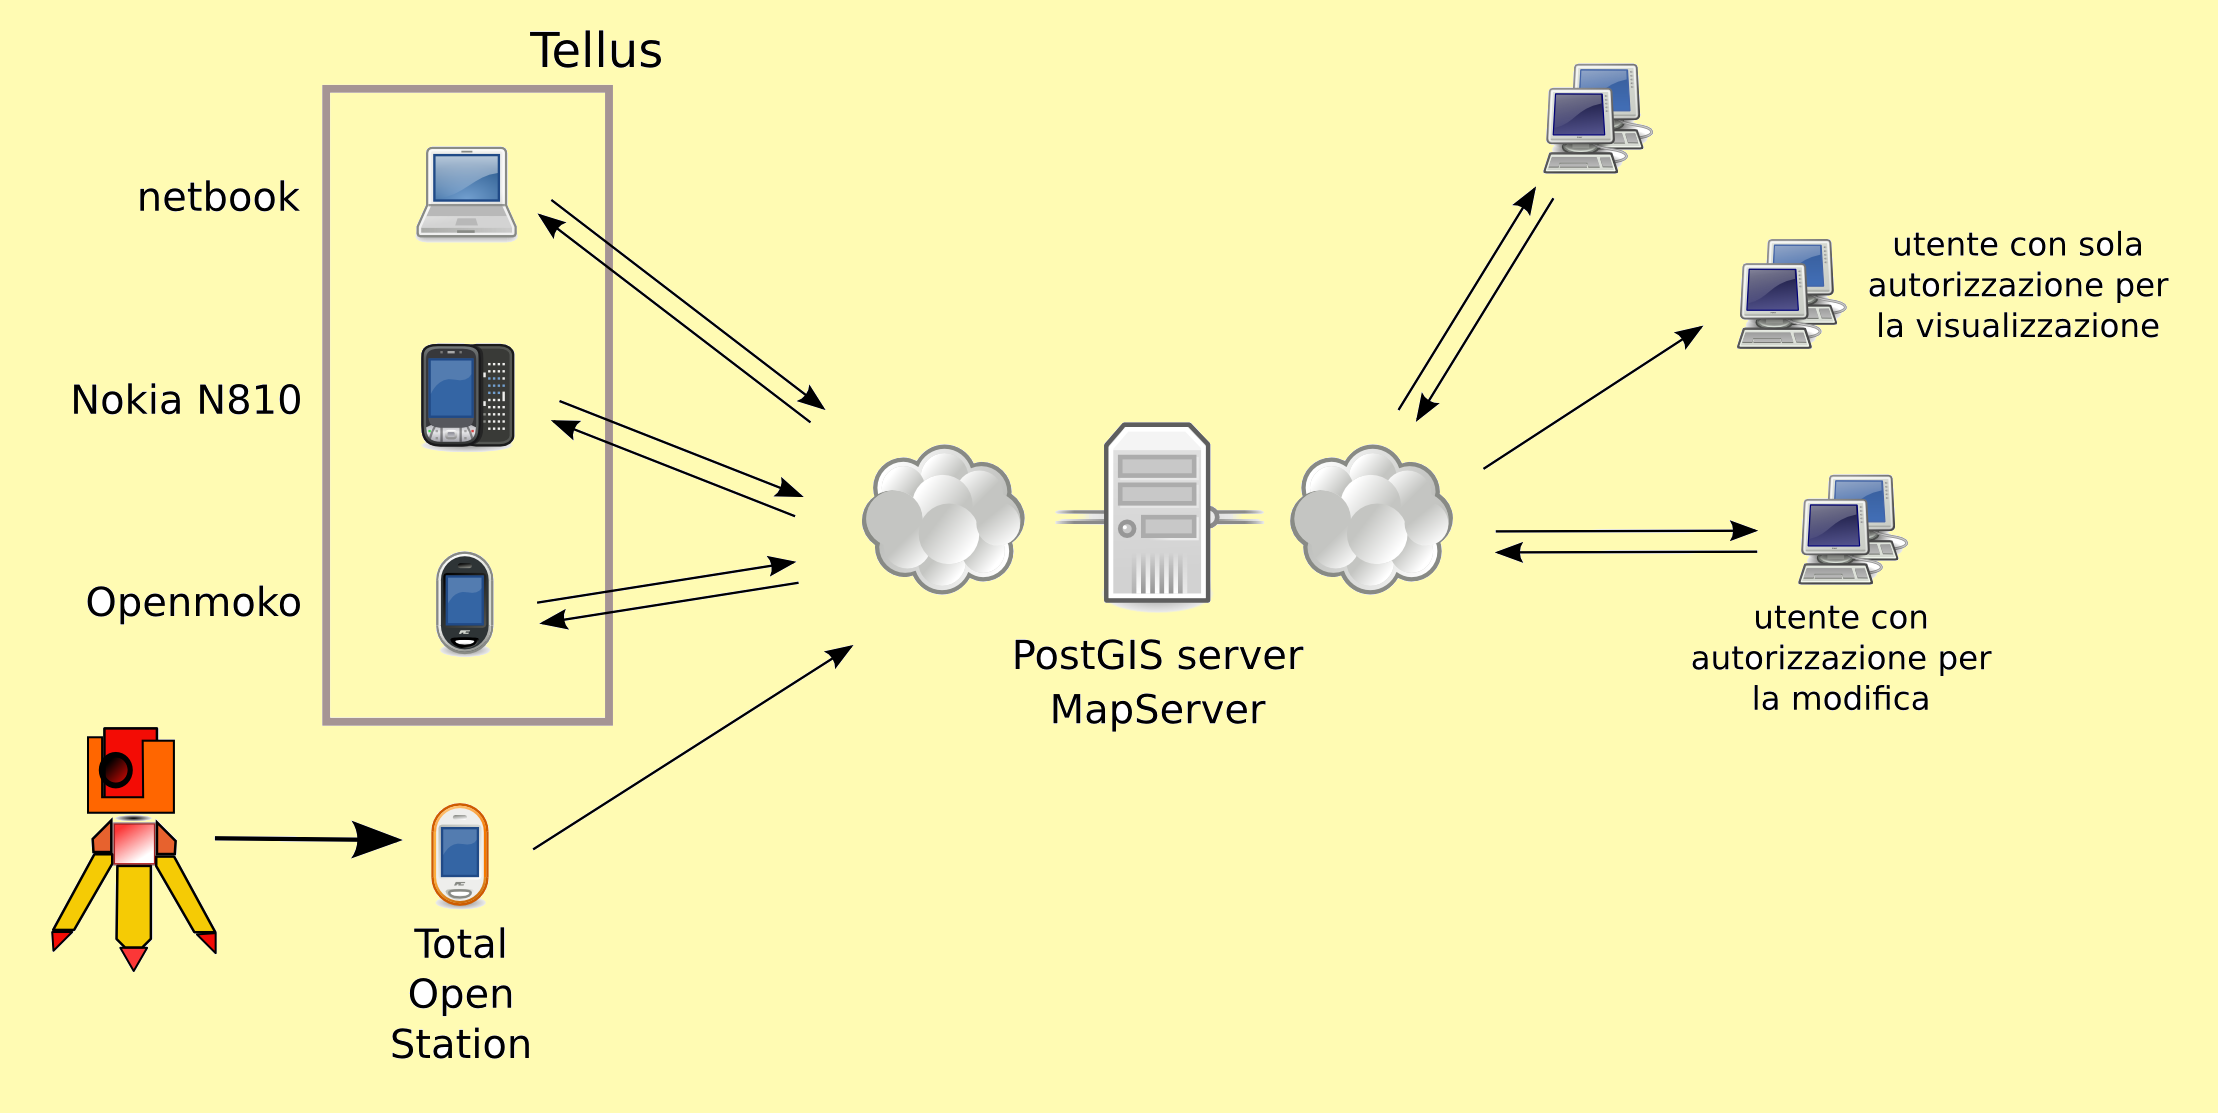
\includegraphics[scale=0.4]{schematellus}
                \end{center}
                \vspace{-20pt}
                \caption{\small{Mobile GIS per l'archeologia (\emph{Francesco de Virgilio}).}\label{schema_tellus}}
                \vspace{-10pt}
            \end{wrapfigure}
        
	Prima dello scavo l'intera cartografia a disposizione, omogeneizzata
	in un formato compatibile con gvSIG e opportunamente
	divisa in layer, viene caricata sul server. Durante le quotidiane
	operazioni di documentazione, il dispositivo palmare connesso
	ad internet scambia in tempo reale informazioni con il server, aggiornando
	simultaneamente i layer vettoriali e raster.

	Il rilievo viene effettuato:
	
	\begin{enumerate*}
		\item con l'utilizzo della stazione totale;
		\item aggiungendo a mano direttamente sul layer del GIS mobile le informazioni.
	\end{enumerate*}

        \begin{wrapfigure}{r}{0.5\textwidth}
                \vspace{-20pt}
                \begin{center}
                        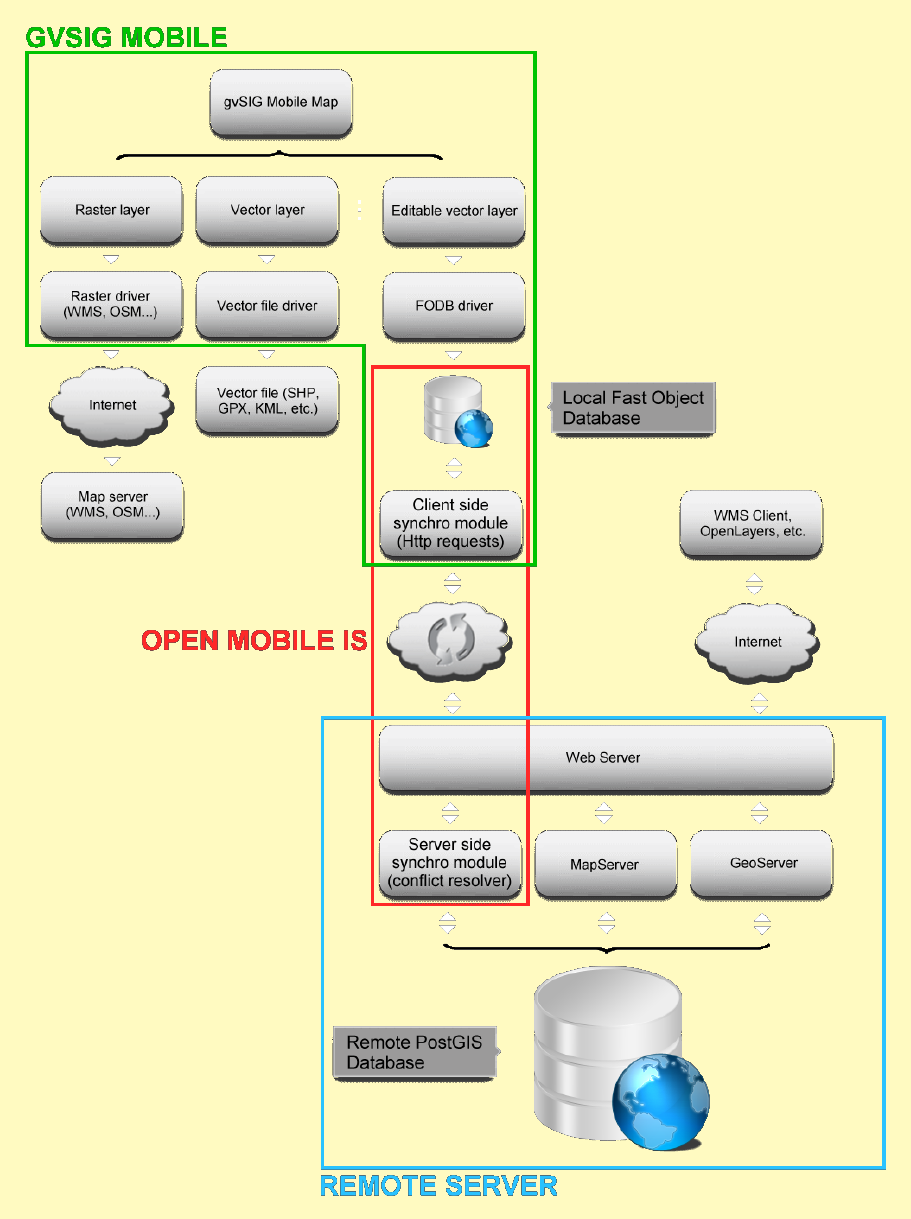
\includegraphics[scale=0.3]{generalscheme}
                \end{center}
                \vspace{-20pt}
                \caption{\small{gvSIG e OpenMIS (\emph{J.L. Dom\'{i}nguez}).}\label{generalscheme}}
                \vspace{-10pt}
         \end{wrapfigure}

	Nel primo caso, non sar\`{a} necessario arrivare nel laboratorio sul campo
	per inviare i dati direttamente dalla stazione totale all'ufficio:
	gli sforzi di Stefano Costa e Luca Bianconi hanno portato alla creazione
	di \textbf{Total Open Station},
	software ben integrato con GNU/Linux per il trasferimento dei dati dalla stazione al palmare via USB, dal quale potrebbero
	essere eventualmente inviati in ufficio via wifi o GPRS.

	Nel secondo caso, tutte le informazioni rilevate vengono sincronizzate
	con il server PostGIS via internet e messe a disposizione dei ricercatori ad esso
	collegati, da qualsiasi punto del mondo.
	Se nel server \'{e} installato ed opportunamente configurato MapServer,
	la cartografia raster viene aggiornata con cadenza regolare, partendo dal database, in maniera tale da poter offrire ai
	ricecatori connessi un WMS quasi in tempo reale, pubblicato sul web tramite librerie open source
        di consolidata funzionalità (ad es. p.mapper o OpenLayers, si veda \textsc{Chaumet}, 2008 e \textsc{Djindjian}, 2008).

	Il dispositivo portatile con Tellus può simultaneamente inviare o ricevere dati, sia in forma vettoriale che raster, poichè gvSIG integra
	il supporto al WMS. Il trasferimento dei dati cartografici tra gvSIG
	mobile, OpenIMS e il server viene effettuato tramite il protocollo
	SOAP (una specifica XML). Il trasferimento effettivo dei file, come si vede in
	fig.~\ref{generalscheme}, pu\`{o} avvenire in due maniere:
	
	\begin{itemize*}
		\item via HTTP, l'intero progetto cartografico viene trasferito in un unico
			archivio;
		\item via Bittorrent, il palmare funge da client e da server
			momentaneo per l'invio dei file cartografici ad altri palmari connessi
			alla rete, sincronizzando i file sull'intero parco macchine portatile;
			agevola la sincronizzazione di grandi quantità di dati,
			perchè ha una migliore gestione della rete e di eventuali
			disconnessioni improvvise.
	\end{itemize*}
  %\vspace{0.3em}
  }

%%%%%%%%%%%%%%%%%%%%%%%%%%%%%%%%%%%%%%%%%%%%%%%%%%%%%%%%%%%%%%%%%%%%%%%%%%%%%%
  \headerbox{Conclusioni}{name=conclusioni,column=1,span=2,below=results neutralization}{
%%%%%%%%%%%%%%%%%%%%%%%%%%%%%%%%%%%%%%%%%%%%%%%%%%%%%%%%%%%%%%%%%%%%%%%%%%%%%%
        Le applicazioni di un sistema portatile di lettura e modifica di dati geografici
	in tempo reale sono molteplici e difficilmente riassumibili. L'applicabilità
	nel settore archeologico \'{e} limitata soltanto dalla connettivit\`{a} sul cantiere, ma offre il vantaggio 
        di unire i momenti del rilievo e dell'elaborazione
	dei dati, operazioni effettuabili da diversi operatori in luoghi differenti, accelerando il processo
	di ricerca e studio del patrimonio archeologico.

%	Si apre al contempo la strada al concetto di \emph{open archaeology},
%	avvicinando il patrimonio archeologico al cittadino, che se non pu\`{o}
%	fisicamente recarsi sul luogo di scavo, potrebbe osservare l'evoluzione
%	della ricerca archeologica quasi ``in diretta'' via internet;
%	in maniera simile, si potrebbe filtrare l'accesso ai soli addetti
%	ai lavori, o distribuire l'analisi su più punti diversi del territorio,
%	o in più centri di ricerca nel mondo.

%	La piena aderenza agli standard \emph{de facto} internazionali dal
%	punto di vista informatico e l'adozione di software open source realizzato
%	in maniera collaborativa, garantiscono la continuit\`{a} del processo
%	di conoscenza, che in questo frangente diventa il filo conduttore
%	tra Archeologia e Tecnologia.\\
  \vspace{0.3em}
  }

%%%%%%%%%%%%%%%%%%%%%%%%%%%%%%%%%%%%%%%%%%%%%%%%%%%%%%%%%%%%%%%%%%%%%%%%%%%%%%
  \headerbox{Bibliografia}{name=references,column=0,below=model}{
%%%%%%%%%%%%%%%%%%%%%%%%%%%%%%%%%%%%%%%%%%%%%%%%%%%%%%%%%%%%%%%%%%%%%%%%%%%%%%
    \smaller
    \vspace{-0.4em}
    \bibliographystyle{ieee}
    \renewcommand{\section}[2]{\vskip 0.05em}
        \textsc{Chaumet A.} 2008, \emph{ Webmapping, arch{\'{e}}ologie et g{\'{e}}oportail}, «Archeologia e Calcolatori», 19, 79-86.\\

        \noindent \textsc{Djindjian, F.} 2008, \emph{Webmapping in the historical and archaeological sciences. An introduction}, «Archeologia e Calcolatori», 19, 9-16.\\

        \noindent \textsc{Gomez M., Delrieu P., Dom\'{i}nguez J.L.} 2009, \emph{The Tellus project}. \vspace{0.3em}

    \textbf{\scriptsize{Quest'opera è rilasciata con licenza Creative Commons CC-BY-SA
    \begin{center}
        \cc\ccby\ccsa
    \end{center}}}
  %\vspace{0.1em}
  }

\end{poster}
\end{document}
